\documentclass[12pt, a4paper]{report}
\usepackage{inputenc}
\usepackage[english]{babel}
\usepackage{amsmath}
\usepackage{amssymb}
\usepackage{minted}
\usepackage{dirtree}
\usepackage{palatino}
\usepackage{syntax}
\usepackage{geometry}
\usepackage[hidelinks]{hyperref}
\usepackage{graphicx}
\usepackage{array}
\usepackage{sidecap}
\usepackage{tikz}
\usetikzlibrary{matrix}
\usepackage{cite}
\usepackage{fancyhdr}
\usepackage{verbatimbox}
\usepackage{titlesec}
% line spacing
\linespread{1.3}

% custom colours
\usepackage{color, colortbl}
\definecolor{Seagreen}{rgb}{0.18, 0.54, 0.34}
\definecolor{Lawngreen}{rgb}{0.48, 0.99, 0}
\definecolor{LRed}{rgb}{1, 0.8, 0.8}
\definecolor{GoldenRod}{rgb}{0.93, 0.65, 0.12}

\usepackage[nottoc]{tocbibind} % put list of... in toc
\usepackage[toc,page]{appendix}
\usepackage{glossaries}
\newglossaryentry{BNF}
{%
    name=BNF,
    description={Backus Naur Form}
}

\newglossaryentry{dependent types}
{%
    name={Dependent Type},
    description={A type whose definition depends on a value}
}

\newglossaryentry{Coq}
{%
    name=Coq,
    description={A proof assistant written in OCaml}
}

\newglossaryentry{parametric polymorphism}
{%
    name={Parametric Polymorphism},
    description={a way of writing generic functions so that they can handle any data type}
}

\newglossaryentry{duck typing}
{%
    name={Duck Typing},
    description={a form of runtime typing where a object is tested for its suitability for a task,
    rather than its exact nature}
}

\newglossaryentry{DSL}
{%
    name={DSL},
    description={Domain Specific Language}
}

\newglossaryentry{lts}
{%
    name={lts},
    description={Long Term Support}
}

\newglossaryentry{ADT}
{%%
    name={ADT},
    description={Algebraic Data Type}
}

\newglossaryentry{strict}
{%
    name={Strictness},
    description={a language is strict if it always evaluates all of the parameters passed to a
    function. A non-strict, or lazy, language, only evaluates what is specifically required}
}

\newglossaryentry{DAG}
{%
    name={DAG},
    description={a directed acyclic graph}
}

\newglossaryentry{totality}
{%
    name={Total function},
    description={a function which has a legal output for every legal input, i.e.\ an output is
    defined for all possible input}
}

\makeglossaries%

%% fake lists inside a table environment
\usepackage{tabu}
\usepackage{booktabs}
\newcommand{\tabitem}{~\llap{\textbullet}~}

%% draw nice frame around code fragments
\definecolor{light-gray}{rgb}{0.9,0.9,0.9}
\setminted{%
    bgcolor=light-gray,
    frame=lines,
    framesep=2mm,
    fontsize=\footnotesize
}  

\setlength{\parindent}{0pt}
\setlength{\parskip}{1em}

%% nice title and chapter formatting
\titlespacing*{\chapter}{0pt}{-40pt}{20pt}
\titleformat{\chapter}[display]
    {\bfseries\huge}
    {\filleft\Large\chaptertitlename~\thechapter}
    {3ex}
    {\titlerule\vspace{2ex}\filright}
    [\vspace{1ex}\titlerule]

%% nice headings for each page
\pagestyle{fancy}
\renewcommand\sectionmark[1]{} %section doesn't set a mark

%% list glossary in toc
\glstoctrue

% ------------------- %
%%  DOC STARTS HERE  %%
% ------------------- %
\begin{document}

%% title page
\begin{titlepage}
  %  \includegraphics[width=\linewidth]{images/ucl_bar_black-eps-converted-to}
  %  \vfill
    \centering
    {\scshape\LARGE University College London\par}
    \vspace{1cm}
    {\scshape\Large MSc Computer Science\par}
    \vspace{1.5cm}
    {\huge\bfseries MicroML \\ A Functional Programming Language for the BBC micro:bit \par}
    \vspace{2cm}
    {\huge\itshape David Kelly\par}
    \vfill
    supervised by\par
    {\large Rae \textsc{Harbird}}

    \vfill
    {\large \today\par}

    \vfill

    This report is submitted as part requirement for the MSc Computer Science
    degree at UCL\. It is substantially the result of my own work except where 
    explicitly indicated in the text.
    
    \vfill

    The report may be freely copied and distributed provided the source is explicitly
    acknowledged.
\end{titlepage}

%% roman numeral
\pagenumbering{roman}%

%% Table of Contents
{\pagestyle{plain}
\tableofcontents
\cleardoublepage}

%% list of figures
{\pagestyle{plain}
\listoffigures
%% list of tables
\listoftables
%% glossary
\printglossaries
\cleardoublepage}


\thispagestyle{empty}
\chapter*{Abstract}
It is increasingly recognized in educational circles that introductory lessons in programming
are a vital part of the modern school curriculum. Programming education in UK has not traditionally
formed a central part of the syllabus. Nearly all teenagers have access to computers and devices, but very
few know how to program them. The raspberry pi has seen a remarkable growth in
popularity since its introduction a mere four years ago. The BBC micro:bit is a project in the
same spirit as the raspberry pi, but with a remit specifically for UK secondary school students.

MicroML is an attempt to bring the fundamental concepts of the functional programming paradigm to
the micro:bit, and thusly to the large body of untapped talent lying in Britain's schools. It 
allows students to explore such ideas as recursive thinking, structural induction, polymorphism
and higher order functions without ever having to be exposed to the underlying theory of such things,
something which no other functional language does.

The project was conceived and written in Haskell. It does not build on any other existing
project. Apart from reliance on standard Haskell libraries all of the major language elements were 
written `ab nihilo', including syntax design, the parser, type inference, repl and compiler.  

MicroML, at point of submission, is a strong base from which to do further work. It has
polymetric type inference, markdown-style inline documentation, a fully-featured repl
environment with extensive error checking capabilities, the ability to check source code for
common programming errors (such as duplicate function definitions and unreachable functions) and
produce images of program callgraphs. It has been designed with the principle aim of making an
environment conducive to learning, without being condescending or overly simplistic. 

\clearpage
\pagenumbering{arabic}
\chapter{Introduction}

\begin{flushright} \textit{`a monad is a monoid in the category of endofunctors, what's
the problem?'} \\ --- not Philip Wadler\footnote{The quote is actually from \textit{A
Brief, Incomplete, and Mostly Wrong History of Programming Languages by James Iry
\url{https://james-iry.blogspot.co.uk/2009/05/brief-incomplete-and-mostly-wrong.html}}, where it is
deliberately falsely attributed, but it is itself a close paraphrase of~\cite{opac-b1078351} p.138.} 
\end{flushright}

\section{Motivation} 
The Wadler quote might be spurious, but a genuine piece of
Haskell documentation drawn from the Control.Monad.Trans.EitherT
library\footnote{\url{https://hackage.haskell.org/package/either-4.4.1.1/docs/Control-Monad-Trans-Ei
ther.html}} available from \textit{Hackage} informs us that `an apomorphism is the generalized
anamorphism for this Monad'. Such statements, while (almost certainly) factually correct are
of little use to the `average' programmer and indeed must be considered to have the effect of
deliberately alienating a large part of the software engineering workforce. One can only hope
that this was not the intention, because functional languages, especially those which use static
type analysis and inference, have a great deal to offer to the programming community in terms
of expressiveness and safety. Must it be the case therefore that introductory material is so
intimidating? Is there a way to encourage students to think functionally, in a type-orientated
manner, without the heavy mathematical `baggage' that is simply surplus to requirements when writing
one's first programs?

\section{Aims and Goals}
\subsection{Project Aims}
It seems only just that a functional language for the micro:bit, assuming that it is not
self-hosting, should be written in a more mature functional language. Haskell was chosen for this
task as it presented a good opportunity to `come to grips' with the language and the paradigm. A
single 10-week UCL elective module in Miranda was not, as anticipated, sufficient preparation for the complexity
of constructing an entire program in a language which is almost aggressive in its focus on purity. 

The primary target, or goal, of the project is to produce, as a proof of concept, the basis of a
language designed primarily for teaching purposes, but practical enough to write real programs for
the micro:bit. Many languages have been implemented over the years with the express aim of teaching
programming concepts. Perhaps the most famous and successful of these is Scheme. However, what they
all have in common is that they are intended for an audience who are already interested in computer
science, or are indeed already computer scientists. Even classic texts, such
as~\cite{Abelson:1996:SIC:547755} and~\cite{Friedman1900} are squarely pitched at a sophisticated audience.
The micro:bit is the opposite: it is for students with no previous programming experience,
students who are not mathematicians, and teachers who are neither mathematicians nor programmers.
Functional programming has a reputation in the programming community for being complex and only for a
special type of person. The aim of this project is to show that this is not necessarily the case.
With this in mind, the aim is to make the language as educational and simple as possible, at the expense 
sacrificed expressiveness. 

Development progressed iteratively. Having no previous experience of engineering a large software
project in Haskell, initial development was largely \textit{ad hoc} and unstructured. Haskell is not
an ideal language for development in this manner. A great deal of time was spent just in understanding 
the principles of state manipulation in a side-effect free language. Luckily, there were a number of 
tutorials which served as the backbone, or perhaps more accurately, embryo, of the final project. 
Traces of these tutorials can still be seen scattered throughout the final codebase. These were 
perhaps both a help and a hindrance, as their original authors had not perhaps foreseen that 
they would be so heavily expanded and built-upon. Strong foundations might have results in a project 
which was more realised, with fewer edge cases and areas where the solutions are not as robust as could be desired.

\subsection{Project Goals}
Formally put, the project's goals in order of importance are 

\begin{itemize}
    \item Create an uncluttered syntax for a functional language. The initial inspiration was a
        mixture of Scheme and Miranda. Scheme was considered the better model for evaluation (but
        not for syntax) as it is very simple and relatively pure. While Scheme lacks such items as algebraic data types
        and pattern matching, it clearly exposes the underlying lambda calculus core.
    \item Write a repl environment for students to explore code and concepts. All modern languages
        ought to have a repl, so that individual snippets of code can be tested without the delay of
        compilation and the increased difficulty of pinpointing errors. The repl environment ought
        to be `friendly' and provide as much assistance to the user as possible. 
    \item Have effective type inference so that students do not need to explicitly type variables
        and functions. While not every functional language has type inference\footnote{Idris, a
        dependently typed language, requires type annotations due to the undecidability of inference of
        dependent types.}, it is a fundamental feature of the ML family. Having type inference means
        that the `truth' of types is not hidden from the student as it would be with JavaScript or
        Python, but the onus of explicit type annotations is also absent.
    \item Compiler to micro:bit-flavoured C++. This part of the project which was most
        pertinent to the micro:bit, but also that which would require the most time to bring to a
        degree where compilation of even complicated programs could be accomplished with safety and
        precision. 
\end{itemize}

\chapter{Context} 
\section{The BBC micro:bit} The BBC micro:bit\footnote{\url{https://www.microbit.co.uk/}} is a
microprocessor device aimed at bringing programming to young adults and teenagers. At present it
supports a number of different programming languages, most visibly \textit{MicroPython, JavaScript}
and \textit{TouchDevelop}. These languages, while mainstream and popular,\footnote{With the
exception of \textit{TouchDevelop} of course.} all fundamentally support the same programming
paradigm, the imperative. Doubtless it is vital for all would-be coders to have knowledge and
experience with the imperative/procedural approach to structuring code, but it is not the only
approach, and perhaps not the best for beginners or those with only a passing interest in coding.
It is the contention of the author that a syntactically simple, (relatively) \textit{pure}
functional language would make for an ideal teaching tool on the micro:bit, allowing the
student to focus almost entirely on the problem domain, and a great deal less on syntax and
`boilerplate'. Functional languages are increasingly being used in every area of real-world
applications. In robotics, a field where the micro:bit has already been used with some success,
there has been some research conducted in the use of the declarative style for low level robotics
programming\cite{frob}. This at least demonstrates that the functional style is applicable to the
problem area, but further research would be required to test the suitability of the micro:bit as
a low-level controller. Certainly, anything which can be programmed in MicroPython could also be
written (possible more briefly and with fewer bugs) in a functional language.

\section{Teaching Languages}
There is a long history of languages designed with the express purpose of teaching rather than
production. These generally fall into two streams of development: reduced versions of established
professional languages, and graphical `drag-and-drop' environments. In general, the visual
programming languages, of which \textit{Scratch} is undoubtedly the most well established, are
intended for a younger age group. On the micro:bit \textit{Microsoft Block Editor} is of this
variety. \textit{Microsoft Touch Develop} and \textit{Code Kingdoms JavaScript} appear to offer a
hybrid experience, with textual code presented in a coloured, graphical editor. Finally there is a
port of the Python programming language, which best typifies that school of tuition where a real
language is used in a simplified context.

\section{Python as Teaching Language}
While Python was not explicitly designed as a teaching language, in recent years it has increasingly
been used as an introductory language in university settings. MIT, where Scheme was first created
and promoted, has begun to teach its introductory courses in Python. With Python already available
on the micro:bit, why is there the need for another text-based language on the same platform? Is
this not just `muddying the waters' of what should be a simple educational tool? Do instructors
really have the time to learn another language in the event that students express an interest in programming
functionally?

In an attempt to address some of these questions, it is necessary to derive some picture of what might
constitute a functional language, and why it might be a useful way to teach programming to younger
learners. Being more a philosophical stance than technical necessity, it is possible to mix various
paradigms together to form \textit{hybrid} languages. In practice, most programming languages take
precisely this approach\footnote{Truly pure languages are a rare thing: in the realms of OOP perhaps
only \textit{Smalltalk} and \textit{Ruby} qualify. In the functional language family, the only
mainstream entirely pure language is Haskell.}. Python, for example, supports a great deal of the 
functional paradigm, as does JavaScript. These already exist on the micro:bit: why not just use those? 
Consider the following simple scenario, we want to sum all the occurrences of the number 3 in the
following list: 

\mint{python}|nums = [2,3,4,3,2,3,5]|

To do this in an imperative manner, something like the following might be written:

\begin{minted}{haskell}
    sum = 0
    for i in range(len(nums)):
        if nums[i] == 3:
        sum += 3
\end{minted}

To solve this in Python using functional concepts, something like this might be used:

\mint{python}|sum(list(filter((lambda x: x == 3), nums)))|

This is clearly an improvement in terms of brevity, and is perhaps a little easier to understand.
The main difficulty here in the physical writing of the code is balancing the parentheses,
but any good editor should be able to do this automatically. The higher order function
\textit{filter} has a fairly clear meaning to any native English speaker. However the rather obscure
use of \textit{list} and, even worse, \textit{lambda} still makes this rather difficult for the
student. A number of topics would need to be explained here which reduce the utility
of this as a teaching example. Why is the syntax still relatively cumbersome? Because Python was
not conceived as a functional language, many of these features have been grafted onto a traditional
imperative substructure, and the syntax reveals this. The equivalent function in Haskell would be:

\mint{haskell}|sum (filter (==3) nums)|

And an even more generic equivalent in Haskell:

\mint{haskell}|sumAllOccurrences p ns = sum (filter p ns)|

where p is any predicate we care to pass in, such as (==3) or (\textless2). The python code does not
prevent someone from passing in junk values (leading to a runtime error) but the Haskell code, with
the addition of a simple \textit{type signature} can easily be altered to only receive integers,
ensuring type safety. This need not be explained to the student in these terms, but they will
benefit from their program not crashing in unexpected and difficult-to-detect ways. 

This is more powerful than the equivalent Python for loop definition, and a great deal more
flexible. Obviously this could also be implemented in Python using filters and lambda expressions,
but it would still need to be couched inside a function definition.\footnote{This is slightly
disingenuous, as a list comprehension, in both Python and Haskell, would work well here. It does
serve to illustrate the general point. Of course, list comprehensions were first introduced in
functional programming languages.}. In this simple example much of the essence of the functional
programming style can be seen. The advantages are clear: fewer lines of code usually means fewer
bugs and less development time. Students can get to solving problems almost immediately, without the
worry (or rather a reduced worry) about the syntactical correctness of their loops, or balancing a
host of nested parentheses.

Haskell is a large and complicated language and not suitable for younger students. Its runtime
is large and complex, and would almost certainly not run efficiently on the micro:bit, even
in a reduced version. Lazy graph-reduction evaluation would rapidly exhaust the memory of the
micro:bit, leading to constant garbage collection in a manner that might be best described as
`thrashing'. Moreover its emphasis on purity has led it to introduce a number of features which,
while theoretically elegant, are complex even for experienced programmers. There is however a family
of other, related, languages, mostly descended directly or indirectly from ML\footnote{Excepting
the Lisp family representatives, \textit{Common Lisp} and \textit{Scheme}.}, which place different
emphasis on parts of the functional paradigm. Monads, monoids and functors, while important concepts
in programming languages, are definitely out of scope for a teaching language to teenagers. The
approach taken by \textit{Miranda}\footnote{See~\ref{sec:lang} for more details.} is that which will
be followed in the suggested implementation, hiding unnecessary detail with the loss of a little
referential transparency.

\section{Research: Literature Review}
With the thought in mind of creating a Miranda style language for the micro:bit, came the necessity
to decide on the technologies and theoretical basis for the language. Being an implementation of the
lambda calculus, it was necessary to choose an axis on the \textit{lambda cube}\footnote{See
Figure~\ref{fig:cube}} for further development. 

As one of the principle learning goals was to develop some skill with Haskell, a number of books and
tutorials were consulted. Of most immediate use for basic programming were \cite{Lipovaca:2011:LYH:2018642}
and \cite{rwh}. For language design and implementation a number of websites were consulted, among which
\cite{scheme}, \cite{diehl} were particularly useful. Two further tutorials deserve special mention
as they gave simplified accounts of algorithm W \cite{algoW} and the usage of monad transformers
\cite{transformers}, both of which were vital to the success of the project.

Many papers were consulted initially while deciding on the best approach for microML's type
system\footnote{These are detailed in the bibliography.}. In practice, very little of this
reading has made it directly into the language as currently constituted, but it is hoped that the
design allows for future development to integrate some of these possible features more easily,
always bearing in mind the intended scope of the language. This was one of the most difficult
design decisions: what had a legitimate place in a language for a simple processor aimed at
beginners, and what could be implemented entirely for the ego and interests of the developer, or because it
was trivial to do? Design decisions based on ease of implementation or to please the vanity of the
designer are correct only be coincidence, and this is a poor way to design\footnote{This recalls
Tony Hoare's `Billion Dollar Mistake'.}. Of great use were~\cite{Pierce:2002:TPL:509043} with its
excellent general account of type theory (and implementation chapters written in \textit{OCaml})
and\@\cite{Pierce:2004:ATT:1076265} with its exploration of type inference in ML\@.

For the rudiments of language design, both\@\cite{spj2} and\@\cite{spj1} were very informative, the
former for the theoretical basis and the latter for its more practical stance. Regarding language
design in general, both~\cite{Harper:2012:PFP:2431407} and~\cite{plp} were invaluable, especially
the latter with its very clear and concrete handling of the topic. Many details of syntax were
inspired by information gleaned from this book.

Compiler implementation has a large body of literature. For background reading on \gls{BNF} and
parsing,~\cite{torc} gives perhaps the clearest, most modern explanation.
\cite{Appel:1997:MCI:248430} is also extremely useful for its more practical approach. This work,
the so-called \textit{Tiger Book}, is available in a number of different languages. The ML edition is
the most pertinent to this project.

\subsection{The Lambda Cube}
The Lambda Cube was introduced by mathematician Henk Barendregt as a visualization framework for
Coquand's calculus of constructions\cite{Barendregt:1993:LCT:162552.162561}. The simple untyped lambda calculus is not
represented.\footnote{\cite{Pierce:2002:TPL:509043} has a slightly different treatment of the axes.}

\begin{figure} % [!h]
    \centering
    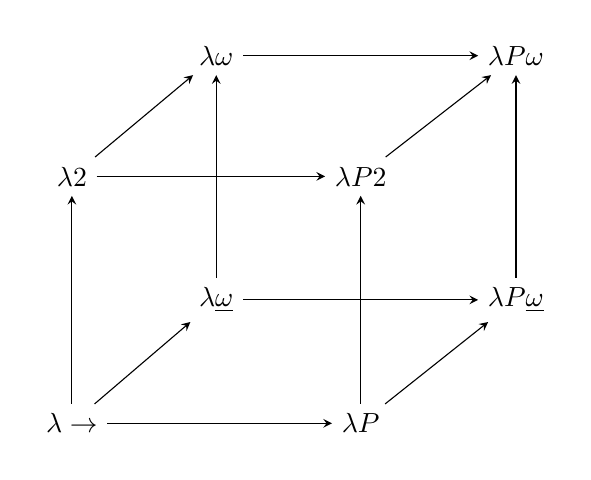
\begin{tikzpicture}
      \matrix (m) [matrix of math nodes, row sep=3em,
        column sep=3em]{%
            & \lambda\omega & & \lambda P \omega \\
            \lambda 2 & & \lambda P 2 & \\
            & \lambda \underline{\omega} & & \lambda P \underline{\omega} \\
            \lambda \rightarrow & & \lambda P  & \\};
      \path[-stealth]
        (m-1-2) edge (m-1-4) % edge (m-2-1) edge (m-3-2)
        (m-2-1) edge (m-1-2) edge (m-2-3)
        (m-3-2) edge (m-3-4) edge (m-1-2) 
        (m-4-1) edge (m-4-3) edge (m-2-1) edge (m-3-2)
        (m-3-4) edge (m-1-4)
        (m-4-3) edge (m-3-4) edge (m-2-3)
        (m-2-3) edge (m-1-4);
    \end{tikzpicture}
    \caption{The Lambda Cube}
    \label{fig:cube}
\end{figure}

This can be understood as exploring refinements of typed lambda calculi. Starting in the bottom
left hand corner $\lambda \rightarrow$ is the simply type lambda calculus as developed by Church,
Curry and Feys in the 1940s\footnote{\cite{Pierce:2002:TPL:509043} p11 gives a simple timeline
of type theory research.}. The top right corner, the `summit' of calculi is $\lambda P \omega$,
which represents \gls{dependent types}. Perhaps no truly practical programming language occupies this
space at present. Theorem provers, such as \textit{\gls{Coq}} have not been used for enterprise software,
and perhaps it is not possible to do so. \textit{Idris}, a dependently typed programming language
written in Haskell, is an attempt to write a general programming language with dependent types. It
is too early in its development at this stage to say whether it will meet with success. A number of
issues, principally the undecidability of type inference over dependent types, would seem to be a
limiting factor to general acceptance.

Naturally, microML makes no attempt to implement $\lambda P\omega$. `Real world' functional
languages, such as Haskell, actually implement hybrid systems which are not represented on the cube.
Most importantly, subtyping (represented as $\lambda F_{<:}$) is missing as a construct from the cube, 
even though almost all language which support record syntax must allow some form of subtyping.

$\lambda 2$, or \textit{System F}, is that system which allows for \gls{parametric polymorphism} (often
called \textit{generics} in such languages as Java and C++)\footnote{See~\ref{appendix:sysf} for
details for a more complete description.}. This seemed a suitable target for microML's type system.
It has the added advantage that there is a well-established algorithm, the Damas --- Milner algorithm
W, which runs in $\mathcal{O}(n)$ time for non-pathological input\footnote{Worst case complexity
for algorithm W actually falls into exponential time, but an input program would have to be both
perversely written and extremely large before this would become a significant liability.}. Type
inference was deemed an important addition to microML as introducing the concept of types, which,
though fundamental to modern computing, carries the risk of rendering it too difficult and different
conceptually from the other languages already available on the micro:bit. These all have in common
so-called \textit{\gls{duck typing}}, and interaction with the type system, programming with types as
it were, is against the nature of the language itself. This is especially true of Python, which
discourages direct type checking on the part of the programmer (though such facilities do exist.).
Good type inference, with easy to read error messages, is an essential feature of microML without
which it would struggle to justify its existence.

\section{Software, Tools, Libraries}
Haskell is ideally suited to the creation of \gls{DSL}s. This is largely due to its
\textit{algebraic data types} which can easily be used to represent the BNF of an embedded
language. Moreover Haskell is blessed with the Parsec library\cite{leijen2001} of parser combinators\footnote{A
\textit{combinator} is simply a function with no free variables, so it only operates on
parameters directly passed to it without reference to any global data within the function
body.}, which removes the necessity of writing lex and yacc files to create a functioning
parser. A parser for another language can be implemented directly in Haskell, using
standard Haskell syntax. Haskell moreover has an extensive library system, located on
\textit{Hackage}\footnote{\url{https://hackage.haskell.org/}}. There is a library for almost any
conceivable requirement. Haskell has two main build tools for project management, \textit{Cabal} and
\textit{Stack}. Neither is as tightly integrated into the language as might be ideal. One need only
compare newer languages, such as Rust and Elixir, where the build tools (Cargo and Mix respectively)
are an integral part of the language, to realize that both \textit{Cabal} and \textit{Stack} have a
rather `grafted on' aspect.

All Hackage packages are available through Cabal, but version management is not
rigorously enforced. Builds can and do break frequently and easily. So-called `Cabal
Hell'\footnote{\url{https://wiki.haskell.org/Cabal/Survival}} is a real problem, especially for
those with no prior experience of the tool\footnote{Indeed, this project was hit twice by Cabal
Hell, once due to a version bump of the ncurses library, and once for a new version of GHC\@.
Some days were lost just to recreate a usable Haskell environment.}. It is poor design to inflict
such problems on an end user who only wants to build a piece of software from source rather then
having the developer subsume them with a dependably build tool. Stack helps in this direction by
maintaining a stable list of packages and creating a strong \textit{sandboxed} environment for
development. The price to be paid is a reduced number of available libraries, so build problems
can still occur with dependencies not part of the \textit{\gls{lts}} system. MicroML was firstly a Cabal
project, but was migrated to Stack later in development. This largely produced a more stable build
and allowed for the use of \textit{intero}\footnote{intero is an alternative to ghci --- the Haskell
interactive environment, but provides better type information and error messages, moreover it has
good integration with neovim, the author's editor of choice.} but unfortunately this also meant that some
experimental code (specially the JIT compiler) had to be disabled. See Section~\ref{SC@2}.

\chapter{Requirements and Analysis}

If the task is to design and implement a functional programming language, the obvious question is:
what is a functional language? Examining some of the leading languages widely regarded as belonging
to the family, a number of features emerge.

\begin{table}
    \resizebox{\textwidth}{!}
    {\begin{tabular}{|c|cccccc|}
        \hline
                    & Pure                    & Lazy Evaluation     & Typing                      & Algebraic Data Types     & Immutable Data          & Closures \\
        \hline
        Common Lisp & No                      & \cellcolor{LRed}Yes & Dynamic                     & \cellcolor{GoldenRod}Yes & No                      & \cellcolor{LRed}Yes \\
        Scheme      & No                      & No                  & Dynamic                     & No                       & No                      & \cellcolor{LRed}Yes \\
        ML          & No                      & No                  & \cellcolor{Lawngreen}Static & \cellcolor{GoldenRod}Yes & No                      & \cellcolor{LRed}Yes \\
        F\#         & No                      & \cellcolor{LRed}Yes & \cellcolor{Lawngreen}Static & \cellcolor{GoldenRod}Yes & No                      & \cellcolor{LRed}Yes \\
        Clojure     & No                      & \cellcolor{LRed}Yes & Dynamic                     & \cellcolor{GoldenRod}Yes & \cellcolor{Seagreen}Yes & \cellcolor{LRed}Yes \\
        Miranda     & \cellcolor{Seagreen}Yes & \cellcolor{LRed}Yes & \cellcolor{Lawngreen}Static & \cellcolor{GoldenRod}Yes & \cellcolor{Seagreen}Yes & \cellcolor{LRed}Yes \\
        Haskell     & \cellcolor{Seagreen}Yes & \cellcolor{LRed}Yes & \cellcolor{Lawngreen}Static & \cellcolor{GoldenRod}Yes & \cellcolor{Seagreen}Yes & \cellcolor{LRed}Yes \\
        \hline
    \end{tabular}}
    \caption{Language comparison}
    \label{tabel:langs}
\end{table}

\textit{Purity} is a rather vexed term than has seen a great deal of discussion in
the literature and on such websites as \textit{reddit}\footnote{For example see
\url{https://www.reddit.com/r/haskell/comments/1874at/io_is_pure/}}. For the purposes of the
following discussion, purity will be considered the ability to write equational code within an
impure framework, where the framework itself can be largely ignored. A Haskell program, for example,
lives within the IO monad. The IO monad is necessarily impure, as it involves interacting with
a system (in this case the operating system) where such interactions are not predicated only on
input data: a system might run out of memory, or experience a power cut for example, which are
events independent or the data. However, on the assumption that the operating system will perform
the actions requested of it, the code running \textit{inside} the IO monad can be understood as
completely referentially transparent. That is, a function called with the same arguments will always
return the same results. This is not necessarily the case with a language like Scheme, which has the
`set!' operator for manipulating global state in a non-transparent manner.

The table shows clearly that there are a few central features which are associated with functional
languages, and other features which are less essential. Bearing in mind the target audience and
the target device, it should be fairly safe to abandon \textit{explicit} monads and
monoids. Why explicit? Natural numbers, for example, are monoidal under both addition and multiplication\footnote{A monoid 
a monoid (or monoid object) (M, $\mu$, $\eta$) in a monoidal category (C, x, l) is an object M
together with two morphisms
\begin{flalign*}
    \mu: M \otimes M \rightarrow M \\
    \eta: I \rightarrow M
\end{flalign*}
Essentially this means there must exist an associative operator and an identity value. For numbers
this might be 
\begin{flalign*}
    1 + (2 + 3) \equiv (1 + 2) + 3 \\
    1 + 0 \equiv 0 + 1
\end{flalign*}
}, but microML will eschew the ability to annotate user-defined types as monoidal instances. Higher
order functions are essential to the paradigm, as is partial function application.\footnote{i.e.\
allowing functions to accept fewer arguments than their arity would suggest. The classic example is
$inc = (+1)$ where the + operator has been partially applied.}

\gls{ADT}s are found in nearly all of the major functional languages. The notable
exception again is Scheme. This is of additional interest in that Scheme is the only language of
those listed which was explicitly designed as a teaching language. It is worth clarifying at this
stage that any complete lambda calculus implementation has the potential to create ADTs, the missing
element is the syntactic sugar provided the sum and product types in languages such as ML and
Haskell. The same is also true of tuples and lists, which do not require special status in a
lambda calculus language, but are often given so for reasons of efficiency and programmer
satisfaction. The immediate application of ADTS for micro:bit programming is not immediately
apparent, so, much in the manner of Scheme, these will not be considered a priority of microML.

\section{Language Design} 
\label{sec:lang}
Miranda\textsuperscript{TM} is a language
created by David Turner in the early 1980s\footnote{The wikipedia page says that Miranda supports
monads. This is not correct, in the sense that it is not possible for the programmer to create
monad instances or explicitly interact with monads. It is also unlikely that Miranda is using
monadic concepts at the implementation level as these were first introduced into Haskell a number of
years after the introduction of Miranda}. It is a member of the ML family, one of the first purely
functional programming languages, and the direct parent of Haskell and Haskell's various offshoots.
Indeed, one of the reasons for the creation of Haskell was the fact that Miranda was trademarked and
closed source. It might best be described as a (small) subset of Haskell\footnote{Though it would
be more accurate to describe Haskell as a superset of Miranda.}. It is still used as a teaching
language and has a very clean, simply syntax. A reduced version of Miranda is suggested for 
the language, which will go under the working title of microML.\footnote{microMiranda would probably be
a more honest name, but there might be a small risk of copyright infringement.}

Miranda has an reasonably rich standard library, which comes loaded automatically in the
interpreter. MicroML should have a subset of this standard library, with functions such as
map, filter and fold\footnote{Miranda distinguishes between left and right folds. This, while
very flexible, might be too complex for most students. Both Clojure and Python have a simple
\textit{reduce} which has the behaviour of a right fold. In Clojure \textit{apply} is similar to
a left fold.}. As far as possible, all built-in functions should be \textit{total}, that is, there
should be no partial functions in the standard library. A partial function is one which does not
produce a legal result for every legal input, for example taking the head of an empty list in
Haskell or Miranda results in a error.

\begin{minted}{haskell}
    head []
    *** Exception: Prelude.head: empty list
\end{minted} 

However this is not a necessity\footnote{The head function in Haskell's standard prelude is a legacy
from Miranda which unfortunately is too late to change easily. The Idris language (itself written in
Haskell) has a built-in function totality checker, usable from the repl, to ensure that such unsafe
practices are deliberate rather than accidental or due to programmer laziness.} and safe versions of
these functions should be written for microML.

Laziness, or more accurately non-\gls{strict}, is an interesting feature of many functional languages, 
but it is a little unclear at the moment what this would mean for programming on the micro:bit. 
Laziness is chiefly useful when dealing with infinite data structures, which is an unlikely
scenario. Moreover, lazy evaluation can make reasoning about the structure of a program more
difficult than is necessary at this stage of the programmer's development, where a more literal
`first this then this' might be easier to understand. 

Another of the more interesting features of the ML family is type inference and static typing.
This is unlikely to be of huge interest to the average student, but it has many benefits. Most
importantly, errors which in a language like Python would only be caught at runtime do not get
past the compilation stage of an ML-style language. Student-friendly (rather than detailed
programmer-friendly) error messages will have to be written to help the student understand what they
have done wrong. Type inference should limit the student's direct interaction with the type system,
which can be very difficult to understand.

Immutability of data is a key (but not universal) feature of the functional paradigm. It allows for
referential transparency and an easier approach to concurrency. Again, these are not features which
are vital to the micro:bit, but they will help students in the future who wish to continue 
coding. Indeed, immutability is in many ways more intuitive for students. If x = 6, then it is 6 for
the entire program. This is a much simpler concept than having a value for x which can go up and down,
or even change type.

\section{Constraints}
The following are the design constraints for microML:

\begin{itemize}
    \item C++ Compiler. The author's initial proposal to MicroSoft was to use an existing Scheme
        to C compiler to turn microML code into something runnable on the micro:bit. It would have
        been relatively easy to convert the microML AST to Scheme. This would have taken advantage of
        the code optimisations and garbage collection of the Scheme compiler\footnote{Either Chicken
        \url{https://www.call-cc.org/} or Gambit-C \url{http://dynamo.iro.umontreal.ca/wiki/index.php/Main_Page}
        would have been suitable choices.}. However, the MicroSoft client preferred a direct
        compilation from microML to C++. This, while perhaps of greater educational benefit, was also
        much more difficult to achieve within the project time frame.
    \item Repl Environment. MicroML should be an interactive experience, with immediate feedback to
        the student. The easiest way to achieve this, rather than constantly flashing to the
        micro:bit and waiting for an error, is to have a repl which the student can use to explore
        concepts and problems. 
    \item Clear Syntax. As far as can be determined, the syntax should be intuitive and simple. That
        is, there should be ideally one way to do things (the antithesis of \textit{Perl's} ethos)
        and to be consistent. For this reason some features, such as function composition, have been
        reinterpreted to allow the student to read from left to right\footnote{Using microML's
        `pipe' operator. See Appendix~\ref{appendix:syntax}.}. The language structure should also
        minimize the number of parentheses needed in an expression.
\end{itemize}

\section{Use Cases}
The primary use case is in schools. The micro:bit has been, or is intended to be, rolled out to
every secondary school in the UK\@. As such it is has not been designed as a commercial product.
MicroML's remit therefore is very narrow, as it only has to target one limited platform with the
express goal of acting as an educational tool. The user is envisaged to be a young adult, between
the ages of 13 and 18, and the instructor, usually a teacher and not a computer science specialist.

\begin{table}
    \begin{tabu}{|>{\columncolor[gray]{0.9}}p{4cm}| p{10cm} |}
        \hline
        Use Case & \textbf{Student Use Case} \\
        \hline
        Participating Actors & Student \\
        \hline
        Flow of Events & \tabitem The student starts with a problem set by the instructor. \\
                       & \tabitem The student opens the repl and explores the problem domain. \\
                       & \tabitem The student creates some working code and copies it to a text file.  \\
                       & \tabitem The student runs the file through the compiler. \\
                       & \tabitem The student passes the resulting C++ file through \textit{yotta} \\
                       & \tabitem The student flashes the binary to the micro:bit. \\
        \hline
        Alternative Flows & \tabitem The student uses a text editor to right code directly. For this
        a simple vim plugin has been provided. At present, only vim is supported. \\
        \hline
    \end{tabu}
    \caption{Student Use Case.}
    \label{table:student}
\end{table}

\begin{table}
    \label{table:educator}
    \begin{tabu}{|>{\columncolor[gray]{0.9}}p{4cm}| p{10cm} |}
        \hline
        Use Case & \textbf{Educator} \\
        \hline
        Participating Actors & Educator \\
        \hline
        Flow of Events & \tabitem The educator invents a problem or uses one provided by the
        curriculum. \\
                       & \tabitem The educator opens the repl and explores the problem domain. \\
                       & \tabitem The educator creates some working code and copies it to a text file.  \\
                       & \tabitem The educator runs the file through the compiler. \\
                       & \tabitem The educator passes the resulting C++ file through \textit{yotta} \\
                       & \tabitem The educator flashes the binary to the micro:bit. \\
        \hline
        Alternative Flows & \tabitem The student uses a text editor to right code directly. For this
        a simple vim plugin has been provided. At present, only vim is supported. \\
        \hline
    \end{tabu}
    \caption{Educator Use Case.}
\end{table}

\chapter{Design and Implementation}
\section{Design}
microML uses an enriched lambda calculus as its base. See Figure~\ref{fig:syntax}

\begin{figure}
    \begin{minipage}[t]{0.5\textwidth}
        \begin{grammar}
            <Expr> ::= Var
            \alt{} Constructor 
            \alt{} Application <Expr> <Expr>
            \alt{} Let Name <Expr> <Expr>
            \alt{} Literal 
            \alt{} If <Expr> then <Expr> else <Expr>
            \alt{} FixPoint <Expr>
            \alt{} UnaryOp <Expr>
            \alt{} BinOp <Expr> <Expr>
            \alt{} PrimitiveErr 
            \alt{} Nil
        \end{grammar}
    \end{minipage}
    \begin{minipage}[t]{0.5\textwidth}
        \begin{grammar}
            <Literal> ::= Integer
            \alt{} Double
            \alt{} Boolean
            \alt{} String
            \alt{} Char
            \alt{} Tuple of <Literal>
        \end{grammar}
    \end{minipage}
    \caption{MicroML's abstract syntax.}
\label{fig:syntax}
\end{figure}

It will be observed that two number formats are supported in the abstract syntax, integers (which in
Haskell are unbounded big numbers) and doubles. The type system however only recognizes a
generalized \textbf{Number}. This decision will be discussed more fully in Section~\ref{sec:type}.

In addition to these basic primitives and control structures, microML also makes use of three
primitives inherited from languages in the Lisp family. Figure~\ref{fig:unary}

\begin{figure}
        \begin{grammar}
            <UnaryOp> ::= Car 
            \alt{} Cdr
            \alt{} Cons
            \alt{} Show
            \alt{} Read
            \alt{} Log
            \alt{} Minus
        \end{grammar}
    \caption{Some of MicroML's unary operators.}
\label{fig:unary}
\end{figure}

These primitives are accessed through the \textit{head}, \textit{tail} and~\:
operator\footnote{MicroML partially follows the example set by Haskell in using~\: for cons. This
was inherited from Miranda but is at odds with the literature, where~\:: is used for cons, and~\: for
has-type.}, which are essential for recursing over lists.

MicroML, in addition to floats and ints, also supports binary, octal and hex numbers\footnote{The
syntax for these is inspired by erlang: one simply writes the number in the form e.g.\ 2\#110 for a
binary 6. Likewise octal is 8\# and hex 16\#}. These are not treated as primitives however, and are
automatically converted to an appropriate numeric representation.

The \textit{FixPoint} primitive allows for the creation of recursive functions by satisfying the equation
\begin{displaymath}
    y\ f\ = f (y\ f)
\end{displaymath}

The most famous fix-point combinator without a doubt is Curry's \textit{Y-combinator}:
\begin{displaymath}
    Y = (\lambda f. (\lambda x.\ f (x x)) (\lambda x.\ f (x x)))
\end{displaymath}

To see how this can be used to simulate recursion\footnote{there are many excellent texts which
give detailed explanations of the \textit{Y-combinator}, such as~\cite{citeulike:2570403}} it is necessary simply
to supply an argument in the form of a lambda abstraction. Figure~\ref{fig:yCombinator}.

\begin{figure}
        \begin{eqnarray*}
            && Y g = (\lambda f. (\lambda x.\ f (x x)) (\lambda x.\ f (x x))) g \\
            & \to_\beta & (\lambda x.\ g (x x)) (\lambda x.\ g (x x)) \\
            & \to_\beta & g ((\lambda x.\ g (x x)) (\lambda x.\ g (x x))) \\
            & \equiv & g (Y g)
        \end{eqnarray*}
    \caption{Y combinator reduction.}
    \label{fig:yCombinator}
\end{figure}

While two different number types are supported by the parser, the type checker only recognizes the
type \textbf{Number}. The compiler will benefit from knowledge of the number type, i.e.\ int or double,
whereas the user (a school-aged student) will not.

\subsection{Parsing}
A number of different libraries were examined before settling on the `standard' \textit{Parsec}
library of parser combinators\footnote{A combinator is a lambda abstraction which contains no
occurrences of a free variable, i.e.\ all of its arguments are explicitly supplied to it, and it
does not rely on any global state or globally defined variables}. \textit{Parsec} is a highly
flexible tool, perhaps more similar to \textit{ANTLR}\footnote{\url{http://www.antlr.org/}} than
to \textit{Yacc} or \textit{Bison}. Explicit, complex-to-read, regular expressions are not required, as the parser
/ lexer is a composite of a great number of small, specialized parser functions, which are linked
together. If one parser fails, the next is tried until either parsing succeeds or a fatal error
occurs.

Other libraries, such as \textit{MegaParsec} and \textit{Trifecta}, both respected and powerful,
were examined. Trifecta especially seems like a very interesting parsing library, with excellent
support for detailed, custom error messages. This would have been ideal for a teaching language
of the nature of microML:\@ unfortunately there is an almost total absence of documentation on the
use of Trifecta, and internet tutorials of any size beyond the trivial do not seem to exist. The
programming language \textbf{Idris} uses Trifecta for its parser, so future iterations of microML
might be able to migrate to Trifecta after careful examination of the Idris source. Moreover,
Trifecta seems to suffer from `Cabal Hell' on a regular basis, as its list of dependencies is
extensive and temperamental\footnote{The author was unable to even install the library without
having to uninstall a great number of conflicting package versions.}.

MegaParsec has excellent support for indentation sensitive grammars, which Parsec does not. Again,
this would be a useful feature to add to microML at a later stage of development. MegaParsec
also have the great advantage that it has the facility to be testing using HSpec\footnote{see
Chapter~\ref{testing}.} whereas Parsec does not allow for automated testing in any Haskell
testing framework. It seems to be, at the present time, misplaced energy to focus on what
is essentially syntactic sugar when other, more vital, elements of the project are still not
as functional as they should be. Moreover, MegaParsec is a relatively new,
and non-standard, library whereas most installations of Haskell ship with Parsec as a component of
the standard library. Of course, eschewing the new in favour of that which is ubiquitous (often
in the name of backwards compatibility) is a bad habit which retards the development of better
software. In this case however, the added power of MegaParsec is not yet required.

Formally, parsec belongs to the family of \textbf{LL(1)} parsers. Obviously this does slightly
reduce the flexibility of the language design\footnote{LL(1) parsers can only recognize a subset
of the context-free languages.}. Haskell itself does not use an LL(1) parser, but rather an
\textbf{LALR(1)} built using \textit{Happy} and \textit{Alex}\footnote{The native Haskell versions
of Lex and Bison.}, much in the manner of a parser constructed using \textit{Yacc}, but such power
is not required for the much more limited range of expression available in microML\. If the language
were ever to be expanded or made more robust, it would perhaps be reasonable to rewrite the parser
to make use of this model.

\subsection{Type Inference}
\label{sec:type}
MicroML uses an implementation of \textit{algorithm W}\footnote{based on~\cite{algoW}.}
for ML-style type inference. At present it is not possible to declare the types of functions, they
can only be inferred. As this is primarily a teaching language with a very simple type system, this
is not the drawback that it might otherwise be.

MicroML is an implementation of \textit{System F}, or the \textbf{second-order lambda calculus}.
It is a typed lambda calculus which supports universal quantification over types, and is thus
the basis for \textbf{parametric polymorphism} in functional programming languages. A full
description of System F is beyond the scope of this report. Interested readers are directed to
\cite{Pierce:2002:TPL:509043} or see Appendix~\ref{appendix:sysf} for a summary. System F is a
`sweet spot' in the lambda cube as it admits relatively easy type reconstruction, which is the basis
of algorithm W.

At a trivial level, primitives have a predetermined type, so \textbf{(Lit (LInt 4))} has type
\textbf{Number}, likewise \textbf{(Lit (LBoolean true))} has type \textbf{Boolean}. At a slightly
higher level, many operators only work on certain types, so the presence of these operators can help
the inference system to resolve the constraints. For example (+) is defined to work only on objects
of type Number. An expression of the type \textit{true + false} will fail with a \textit{unification
error} as (+) is not a supported operator for this data type.

Hindley-Milner is guaranteed to give the most general type signature possible. For example, the
\textit{higher order} function `compose'\footnote{Represented in Haskell by the $\circ$ operator }
has type (Figure~\ref{fig:typesig}).

\begin{figure}
        \begin{flalign*}
            compose : \forall\:a\:b\:c.\;(a \rightarrow b) \rightarrow (c \rightarrow a) \rightarrow c \rightarrow b \\
            let\;compose\;f\:x\: z = f (x\:z)
        \end{flalign*}
    \caption{Inferred type signature and microML definition for `compose'.}
    \label{fig:typesig}
\end{figure}

For readability's sake, the repl uses the words `for all' rather than the $\forall$ symbol. This
informations is suppressed in \textit{ghci}. Testing with students needs to be conducted before it
is possible to say whether the precision of the `for all' comment outweighs the need to explain it.

MicroML has a unified \textbf{Number} type for inference, even though the underlying AST stores
appropriate information regarding the exact form of representation. Miranda too features a unified
number type, with automatic overloading of operators and numeric functions. This makes the interface
a little easier to use initially, as explicit casting is not possible within Miranda. Haskell
overcomes this problem with the use of \textit{type classes}, but this is too sophisticated a
method for microML.\ The loss of detail regarding the types of numbers is unfortunate, but was
considered expedient in the design so as to introduce more basic concepts of type, rather than
computer representation. As such, microML features a limited form of \textit{ad hoc polymorphism}
as related to operator overloading. It is not possible however for students to overload built-in
operators, or define operators of their own\footnote{Untrammelled operator creation can lead to
chaos: the Haskell \textit{Lens} library exports over 100 different operators, leading to code that
can look like the proverbial `alphabet soup'. Such flexibility is useful in a research language, but
introduces a terrible level of extra complexity in a production language.}.

\subsection{Evaluation in the Repl}
The microML repl environment is fully capable of evaluating every aspect of microML's syntax. As
such is can be used either as a simple calculator, or to explore such advanced concepts as closures
and continuation-passing style. The repl has a number of features to make it easier for students to
use, including the ability to request the type of a function, to browse loaded functions, to import
elements from the standard library\footnote{see Section~\ref{libs}} or load user-defined scripts.
It also has intelligent autocomplete for keywords and functions and the ability to scroll back
through past history of the present and previous sessions. Interactions with the repl also feature
syntax highlighting in stdout in an effort to make the content more easily parsed by a student. It
is recognized that the terminal is no longer an environment with which most students are at all
familiar: even many programmers avoid its use. Every effort has been made to make it a pleasant
experience.

\subsection{Floating Point Representation}
\label{floatingPoint}
Haskell uses the IEEE double-precision floating point format\cite{citeulike:3760678}.
This is doubtless very useful for a real programming language, but it would be difficult, and
unnecessary, to have to explain the representation of a number such as $0.1210000000001$ when the
student was expecting to $0.121$. In a similar spirit, a student expecting to see $0.9$ will
inevitably be confused by $0.8999999999$, even if this is an accurate representation of the number
\textit{for the machine}. It was decided to `hide' this implementation detail from the student by
passing doubles through a filter function \textit{truncate'} before printing to the repl. See
Appendix~\ref{appendix:samples}.

\subsection{Comments} MicroML also features a small embedded language, a DSL
within a DSL for commenting files. This language is a simple variant on the
textbf{markdown}\footnote{\url{https://daringfireball.net/projects/markdown/}} markup system. See
Appendix~\ref{appendix:md} for the syntax. A separate parser was written for a small subset of
markdown and pretty printing facilities for the terminal. It is assumed that the terminal is capable
of rendering standard ascii escape sequences. Figure~\ref{fig:comments} illustrates a typical
encounter with the comment system.

\begin{figure}
    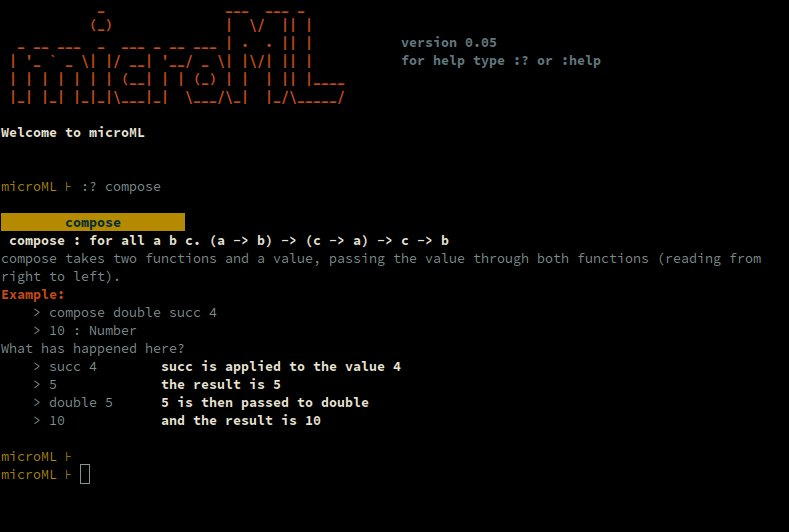
\includegraphics[width=\textwidth]{images/comment.jpg}
    {\caption{Comments as seen in the terminal}}
\label{fig:comments}
\end{figure}

In addition to help regarding function definitions, there is also a glossary of terms for those new
to programming. Terms in the glossary are underlined in the main commentary text.  Another teaching 
tool which has been added to the repl environment and which the author believes to be unique
is the ability to print the parse tree of an expression within the repl. See figure~\ref{fig:tree}.

\begin{SCfigure}
    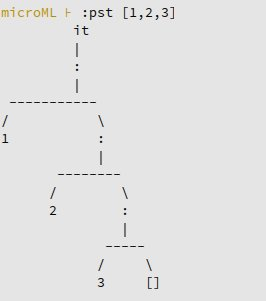
\includegraphics[scale=0.6]{images/tree.jpg}
    {\caption{Parse tree of a simple expression as viewed in the terminal}}
\label{fig:tree}
\end{SCfigure}

The parse tree can also be printed out as a text string, in the form that it is constructed and
de-constructed by the parser/evaluator. Figure~\ref{fig:parsetext}

\begin{figure}
    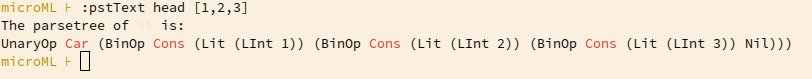
\includegraphics[width=\textwidth]{images/parsetext.jpg}
    {\caption{The text string of a parsed expression}}
    \label{fig:parsetext}
\end{figure}

\subsection{Programming Style}
It is the intention of microML to encourage modularity of design, aiming at function composition
above all. Large, complex functions are to be actively discouraged in favour of smaller, more
`mobile' units. Both Haskell and Miranda contain a function composition operator, a single dot.
This is inspired directly by the mathematical notion of composition, where it is notated $ f \circ
g $. While it is doubtless more mathematically pure to copy this approach, the expected user of
microML is not a graduate mathematician, and probably only has GCSE level of maths, if that. MicroML
follows the model of \textbf{Elixir} with its left-to-right \textit{pipe} operator $|>$. However
microML prefers the notation $>>$ as being more explicitly about direction and movement.

\section{Implementation}
MicroML is written in Haskell and microML itself. However it should be stated that this is not the
pure Haskell of the 2010 report\cite{Marlow_haskell2010}, but makes use of a number of extremely
useful extensions provided by the Glasgow Haskell Compiler, GHC.\ This unfortunately does limit the
portability of microML, but it would be reasonable to say the GHC has largely become the `de facto'
Haskell implementation, moving the language as a whole more in the direction of the Python model,
which is defined by CPython, rather than a formal document description.

In addition to the main program, there is also a simple vim plugin with syntax highlighting,
comment folding and a primitive autocomplete, which makes editing microML in the editor a slightly
more pleasant experience. Granted, it is a little at odds with the stated objective of microML ---
which is ease of use and suitability for beginners --- to promote vim as \textit{editor of choice} but
this was largely convenience for the author whose preferred editor is \textbf{neovim}, an ambitious
refactoring fork of vim.\footnote{\url{https://neovim.io/}}

External dependencies to the main program are deliberately few. An experimental JIT
compiler makes use of LLVM\footnote{\url{http://llvm.org/}} with the associated Haskell
bindings\footnote{Unfortunately the bindings are still only for LLVM 3.5, whereas the
upstream version of LLVM is now 3.8. For this, and other reasons to be discussed, JIT
compiler development was suspended for this first microML deliverable.}. The compiler
also makes optional use of \textbf{clang-format}, a command line utility available with
\textbf{clang}\footnote{\url{http://clang.llvm.org/}} for formatting the generated C++ code. The
graphics program \textbf{graphviz}\footnote{\url{http://www.graphviz.org/}} is also used (again
optionally) for producing \textit{png} files of a program's callgraph.

Handling state in Haskell is by no means trivial, and does not allow for easy prototyping. One needs
to understand exactly how to structure a solution to a problem before embarking on development,
otherwise one risks having to rewrite large sections of code when it becomes apparent that a
particular function needs to reside inside a particular monad, and does not. For example it is not
possible to trivially wrap a function in a \textit{try / except} clause as one would in Python.
Anything which might through an exception needs to be inside the ExceptT monad transformer. The type
checker will reject anything else. This can be sidestepped to a certain extent by throwing an
unchecked \textbf{error}\footnote{a wrapper around the prelude library function \textbf{undefined}},
but such an error kills the runtime system, crashing the program.\footnote{\cite{transformers} was
invaluable for understanding the monad transformer abstraction.}

To successfully combine state with error handling it is necessary to `string together' various monad
transformers over a base monad type. While this is an elegant solution and makes writing pure code
easier, it is by no means obvious how to create these initial `stacks' of monads. The advantage
however is that, once the complexity of stack construction has been overcome, this complexity is
`locked away' within one or two data types and functions, allowing the programmer essentially to
forget about state management and error handling details. 

\subsection{False Starts \& Dead Ends}
\label{deadend}
Some libraries and approaches were abandoned during the development process. Most notably a deal of
time was put into using the \textit{Language-C} library for manipulating the C AST in Haskell. While
this would certainly be the robust approach for writing the C code generation element of microML,
it was decided that time constraints did not allow for proper utilization of the library (which is
very large) so other alternatives were explored in the hope of at least producing a testable backend
within the time frame of the project. Moreover the library is strongly inclined to C, rather than
C++, so many bindings are completely missing, including some data types and all object-orientated
code constructions. There is no equivalent library for C++ on Hackage. This remains to be written. 

\subsection{Project Structure}
Every effort was made to organize the source code in a logical and consistent manner, such that
another programmer should understand the organization without great difficulty.
Figure~\ref{fig:dir}.

\begin{figure}
    \dirtree{%
        .1 microML.
        .2 docs.
        .2 src.
        .3 Compiler.
        .3 Jit.
        .3 Libs.
        .3 Main.hs.
        .3 MicroML.
        .4 Typing.
        .3 Repl.
        .2 test.
        .3 compiler.
        .2 utils.
        .3 vim-mmlFold.
        .3 mml.vim.
        .2 microML.cabal.
        .2 stack.yaml.
    }
\caption{Directory Structure}
\label{fig:dir}
\end{figure}

\subsubsection{JIT}\label{JIT}
The inclusion of a JIT aspect was predicated on an experimental method to produce C++ code using
the existing LLVM compiler framework. The JIT compiler makes use of the LLVM 3.5 bindings available
from \textit{Hackage}\footnote{\url{https://hackage.haskell.org/package/llvm-general-3.5.1.2}}.
LLVM is capable of outputting a C++ file, in addition to machine code or the LLVM \textit{IR}.
An online tutorial\footnote{\url{http://www.stephendiehl.com/llvm/}} formed the basis for the
experiment. It was felt that LLVM might be able to produce suitable code for the micro:bit, with
optimisations well out of scope for a simple nano-pass compiler such as has been implemented. The
JIT was abandoned during development however when it became clear that the generated C++ code was
too heavily indebted to the LLVM environment. While the code was correct, it would not compile under
\textit{gcc} without heavy, intelligent, editing. It was deemed more difficult to render the code compilable
with \textit{yotta}\footnote{\url{http://yottadocs.mbed.com/}} than it would be to simply write a
simplistic naive compiler.

\subsubsection{Compiler}
The compiler makes a single pass over the source file, and does not utilize an intermediate
representation. Some error checking and simple optimisation is performed however. The compiler
conducts a number of tests on the source code before attempting a translation into C++. First the
code is searched to ensure there is a main function. In the repl, there is no necessity of a clear
entry point, but a compiled file needs to have a clear and defined structure. If a main function is
found not to exist, an appropriate error message is issued. Moreover, the compiler searches for
duplicate definitions. This is partially to check for carelessness on the part of the student, but
also to help enforce data immutability. Top level re-declaration of values is rejected by the
compiler. Perhaps the most interesting feature of the preprocessing phase is found in CallGraph.hs.
The source code is analysed and converted to a \textit{\gls{DAG}}. This is then
searched, using a depth first search algorithm, to discover all functions reachable from
\textit{main}. If any function, or functions are found to be unreachable, compilation is abandoned
and a message is issued describing the procedure for creating a callgraph.png. See
Figure~\ref{fig:callgraph}.

\begin{figure}
    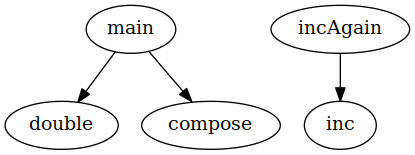
\includegraphics[width=\textwidth]{images/callgraph.png}
    {\caption{A example callgraph for a simple program. This would fail to compile.}}
    \label{fig:callgraph}
\end{figure}

Code generation is done in much the same manner that the repl performs evaluation, but instead of
reducing each term to normal form, it translates them to statements and expressions in C++. 

\subsubsection{Repl}
The repl is probably the most fully realized interface to the language. Perhaps the most interesting
feature is its handling of multiple states with a custom datatype. 

\begin{minted}{haskell}
    data IState = IState
        { typeEnv :: Env
        , termEnv :: TermEnv
        , helpEnv :: HelpEnv
        }
    type Repl a = HaskelineT (StateT IState IO) a
\end{minted}

The Repl monad carries with it three separate hashmaps, holding stateful information regarding the
types of functions, the function definitions, and the help environment. This last is not accessible
for writing from within the repl, but only via loaded file.

\subsubsection{Libs}
\label{libs}
MicroML ships with a limited standard library. Functions in `standard.mml' are automatically loaded
in the repl environment and are always available in the compiled environment. Other libraries need
to be loaded manually with the `:using' command. The libraries available at time of writing are:

\begin{itemize}
    \item standard: a large number of utility functions, modelled on the standard library available
        with Miranda (though less extensive). Students are not expected to be able to write their
        own implementations of `map' or `foldr' so these have been made always obtainable.
    \item Maths: the maths library contains some constants, such as $e$ and $\pi$, some utility
        functions such as `floor', `ceiling' and `intToFloat' and typesafe logarithmic functions.
        These last are wrappers around Haskell's `logBase' function.
    \item string: as strings are literals in microML, they need their own library to allow for
        manipulation. At present there are a few functions for converting between upper and lower
        case and obtaining the ascii value of a char. This library is nascent and needs to be
        expanded.
    \item combinators: a library for those interesting in the pure untyped lambda calculus. The
        functions presented here include $s$, $k$ and $i$, which themselves constitute a
        \textit{Turing complete} language and a number of other combinators, including those
        introduced by David Turner in his seminal paper~\cite{TUR79a}.
    \item church: this is another library dedicated to the underlying lambda calculus, presenting
        natural numbers as functions using \textit{Church encoding}\footnote{\url{https://en.wikipedia.org/wiki/Church_encoding}}.
        This is primarily intended for those students who display an interest in understanding the
        evaluation model of microML\@.
\end{itemize}

\chapter{Testing}
\label{testing}

Software testing is a vital part of any seriously intended development project. Only an arrogant
programmer, or one of little experience (often the two go together) would claim that a function or
module had been written without mistakes, or that all edge cases had been properly handled. It is
difficult for a human to be ruthlessly systematic: precisely the approach that testing needs, and
precisely that which a computer does with ease. Thankfully Haskell has a number of powerful testing
frameworks, making the writing of unit tests especially simple. Both \textit{Cabal} and
\textit{Stack} support integrated testing, making the process of running tests and building trivial.

There are four generally recognized levels of software testing. Unit testing is the examination of
individual methods or functions to ascertain that they behave as expected under a variety of
conditions. This type of testing is best conducted during software development, in concert with the
writing of the actual executable. Integration testing ensures that individual modules (or
classes) work together as expected. This is one level of abstraction higher than unit-testing.
System testing looks at the functioning of the entire system, and finally acceptance testing sees
whether the end product will be suitable to the client. MicroML has not been acceptance tested, and
still requires work in this direction.

The Hspec\footnote{\url{https://hspec.github.io/}} package focuses primarily on unit testing of
Haskell functions. Real \textit{TDD} would have seen tests written in parallel with production code:
due to the lack of experience the author had with Haskell at the beginning of the project, this was
not the development method deployed as it would have been too heavy a cognitive burden in addition
to wrestling with various problems of type, state and program structure. Unit tests were written
after the fact, and, at time of writing, do not yet have full coverage of source code.

To run tests while building it is necessary simply to enter in the terminal the command `stack test'
while in the project root directory, which is equivalent to building and testing the
software.

Testing the ability of the compiler to produce C++ code involved the addition of integration tests
to the Hspec framework. These are handled separately in the form of multiple small \textit{mml}
files. A simple bash script runs each file individually through the microML compiler. At time of
writing, the compiler does not yet successfully pass all of these integration tests. More work needs
to be done before the compiler can seriously be considered to be `fit for purpose'. The script must
be run from the utils folder of the project.

\chapter{Conclusions and Project Evaluation}

\section{Achievements}
The project has met all of the goals and requirements initially specified, but this is not to say
that the project cannot be improved or could even, in any real sense, be said to be finished. The
syntax (see Appendix~\ref{appendix:syntax}) is clean and uncomplicated, but also quite limiting for
students who would like to be more `expressive'. It is felt that, for those advanced students who
find microML to be a tad stifling, there already exist a large number of more powerful languages
which they can go on to explore, not least of which is Haskell itself. 

MicroML supports both ad-hoc polymorphism and full parametric polymorphic type inference. As such
it can be considered a complete implementation of \textit{System F}. This could be extended to
make it more flexible, e.g.\ sum and product types. The lack of subtyping might be considered a
drawback in a genuine language. It would be theoretically pleasing to allow students to access the
implementation details of number types, constraining user-defined functions to integer or double.
This is not presently possible for functions written by students. It is possible for
system-defined operators and functions. For example the modulo `\%' operator will throw an error
if either of its operands are not integer literals. This is `hard-coded' into the inference engine,
which is unfortunate. Figure~\ref{fig:modulo}.

\begin{figure}
    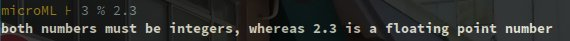
\includegraphics[width=\textwidth]{images/modulo.jpg}
    \caption{Type error with modulo operator}
\label{fig:modulo}
\end{figure}

The compiler element of the project successfully compiles many simple programs written in microML,
including the traditional `hello world'. The repl is a fully-featured environment than exceeds the
capabilities of many `professional' languages. Its error messages (the same which appear in the
compiler) and syntax-highlighted and written in `plain English'. Figure~\ref{fig:typeError}

\begin{figure}
    
\includegraphics[width=\textwidth]{images/typeError.jpg}
    \caption{Unification error}
\label{fig:typeError}
\end{figure}

\section{Evaluation}
At the fundamental design level, perhaps the most unfortunate decision was to make the \textit{Expr}
datatype a simple type with kind \textit{*}\footnote{* is pronounced `type'.}. This decision
has meant that it was not possible to make \textit{Expr} an instance of the \textit{Functor}
typeclass\footnote{A datatype needs at least kind $* \rightarrow *$ to be a member of the
Functor typeclass.}, meaning that a complex expression was neither mappable nor foldable. There are
instances in the code where expressions have been converted into strings via `show' in order to
filter or search for elements. This is rather inefficient and, given the nature and complexity
of regular expressions, potentially bug-prone. This problem would have been alleviated by a
definition for `fmap'. Once \textit{Expr} is a functor, it would then be relatively trivial to make
a traversable instance, and even, if necessary, a monad instance, or at the very least an instance of
\textit{Applicative}. Tag information regarding type could have been carried in the additional arity
required by the functor typeclass. \textit{Expr} would then have kind $* \rightarrow *$ with the
first * being a type primitive. This would also have made inference easier and quicker. However it was
nearing the end of the project before the author had enough knowledge and skill to be aware of these
subtleties, and such a change would require a rather substantial rewriting of much of the MicroML
module.

\section{Future Work}
While the basic core of the language is largely complete a great deal of work remains to be done on
the compiler and making the language more usable as an educational tool. As a number of features
were included in an unfortunately \textit{ad hoc} manner, integration is not as tight as might be
desired. An obvious case of this is the existence of two separate parsers, one for mml source code,
and another for documentation. This has resulted in a rather fragile relationship between the two,
and an over-sensitivity to context (especially around the existence of unanticipated whitespace)
and code duplication in the Repl.Repl module. It also entails two passes over a source file, which
is wasteful of computer resources and time. A future iteration would seek to unite these into one,
more robust parser. Regarding the parser, it might also be a possibility to make it indentation
sensitive. This could result in more readable source files for students. However, one of the stated
aims of microML is to encourage piping of small functions (in the manner of the unix pipe) rather
than building large functions. An indentation sensitive parser might actively encourage the growth
of function complexity. Further investigation would be required before a definitive decision could
be reached.

The present approach to C++ compilation, while valid as a proof of concept, is perhaps not
sufficiently robust to allow for genuine expansion to the level of complexity which might be
required of it. Alternative, better, strategies would involve direct translation of the microML AST
to the C++ AST, enabling the compiler to perform optimisations. Apart from checking the validity of
the source file, the compiler is unable to conduct optimisation routines. Time has been the single
greatest factor in limiting the efficacy of the compiler element of the project. There is a library
for the manipulation of C code in Haskell~\ref{deadend} but there is nothing specifically for C++.
Either the existing library would have to be modified to allow for class manipulation and the
micro:bit's \textit{managed types} or a new library would have to written. This is far beyond the
scope of the present project, but would seem to be a necessary step to render the compiler a more
industry standard product.

Related to the compiler is the issue of \textit{memory management} on the micro:bit. The API already
exposes a number of managed types which do not require manual freeing, but microML supports closures
and also could be made to support \textit{continuation passing style}, both of which would need to
claim space on the heap and therefore need freeing at some point. A simple \textit{mark \& sweep}
garbage collector is used by microPython. The memory management process for the JavaScript
implementation is not open source. Experiments with microPython have revealed that the garbage
collector takes too much of the available memory for itself. On such a constrained system this can
lead to problems when attempting to use the inbuilt censors or bluetooth. An alternative might be
the use of a \textit{region inference algorithm}\cite{Tofte:1998:RIA:291891.291894}. Work on
MLKit\footnote{\url{http://www.elsman.com/mlkit/}} has shown that region inference memory management
can, at least sometimes, act as a realistic replacement for garbage collection. In a system where
programs are expected to be relatively uncomplicated, such as on the micro:bit, this might be an
ideal `fit'.

Of features missing from the language definition itself, the most obvious omissions are
\textbf{pattern matching} and \textbf{algebraic data types}. The absence of ADTs has already been
discussed, but their presence would be most useful for writing of standard library modules. Without
ADTs the creation of new data structures, while possible, is far more difficult than need be.
Pattern matching is largely syntactic sugar for nested \textit{if --- else if} clauses, and indeed
is desugared in Haskell to nested case statements. A student using microML can simply write such
things themselves, but the ubiquity of pattern matching syntax suggests that it ought to be included
in the language at some point, even if it cannot be regarded as a \textit{primitive} of the
functional style. 

Another important feature at present only partially implemented is user-defined
exceptions\footnote{the parser and typechecker recognize the syntax, but the evaluator and compiler
do not}. The approach in~\cite{deGroote1995} to a lambda calculus of exception handling would make
for an area of further interesting study, allowing exceptions to be thoroughly integrated into the
existing language.

The type inference system is compliant with \textit{System F}. While this is not the most demanding
of type environments within which to work, it might still be too rigid for students with no
programming experience at all, and represent a barrier to entry. Real world programming languages
tend rather to use a variation on $F_{<:}$\footnote{Pronounced F-sub. This allows for subtyping:
a function could be made to accept only a Double, or a general Number type, where Double and
Int are subtypes of Number. This is both a more flexible and powerful type system, and one used
by many real world languages.}. MicroML might be more successful and usable if, rather than
extending a simple type system as it does at present, it might instead use a restricted form of
a more complex lambda calculus. Future work might also examine the possibility of delaying, or
\textit{proroguing} type checking until the student has fleshed out an approximate solution to a
problem\cite{Afshari:2012:LPP:2384592.2384595}. Type-checking then becoming an interactive tool
for improving software, rather than an overly tight straitjacket it can seem for those not used to
moving within its constraints.

If such a prorogued system could be implemented, then it might be possible to `climb the lambda
cube' as it were. A student could first program dynamically, with duck typing in the manner of
Python, then refine the program to be compliant with System F. It might thereafter also be possible
to increase program safety and security by introducing elements of dependent types where
appropriate. This incremental approach to static typing could encourage students to work with the
type system rather than feel they are fighting it. Even a partially dependently-typed program could
result in a number of possible compiler optimisations and greater runtime safety.

%% appendices
\begin{appendices}
    \chapter{Installation Guide}
    To build and install microML on a *\textit{Nix} system there is an installation script in the main directory
of the repository. This does not need to be run with sudo permission. See
Appendix~\ref{appendix:samples}.  To build and install microML ensure that
\textbf{stack}\footnote{\url{https://docs.haskellstack.org/en/stable/README/}} is installed. 

\textbf{MicroML has not been tested on Windows.} 

\begin{figure}
    \label{fig:help}
    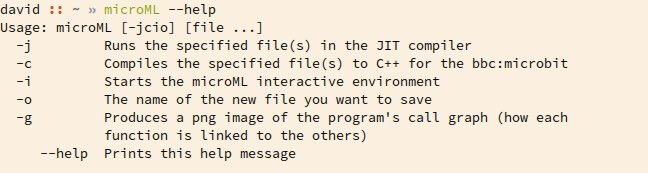
\includegraphics[width=\textwidth]{images/help.jpg}
    {\caption{MicroML command line help}}
\end{figure}

\begin{itemize}
    \item Download the repository from Git \url{https://github.com/kellino/microML}
    \item Unzip the repository and cd into the directory.
    \item run installMicroML
\end{itemize}

Assuming the build has been successful, typing `microML --help' into the terminal shows the various options. See Figure~\ref{fig:help}.



    \chapter{System F}
    \label{appendix:sysf}
    This treatment of System F is taken from~\cite{Pierce:2002:TPL:509043}

\begin{minipage}{0.4\textwidth}
    \begin{tabu}{l l r}
        t ::= & & \\
              & x & \textit{variable} \\
              & $\lambda x:T.t$ & \textit{abstraction} \\
              & t t & \textit{application} \\
              & $\lambda X.t$ & \textit{type abstraction} \\
              & t [T] & \textit{type application} \\
    \end{tabu}
    \begin{tabu}{l l r}
        v ::= & & \\
              & $\lambda x:T.t$ & \textit{abstraction value} \\
              & $\lambda X.t$ & \textit{type abstraction value} \\
    \end{tabu}
    \begin{tabu}{l l r}
        T ::= & & \\
              & X & \textit{type variable} \\
              & $T \rightarrow T $ & \textit{type of functions} \\
              & $\forall X.T$ & \textit{universal type} \\
    \end{tabu}
    \begin{tabu}{l l r}
        $\Gamma$ ::= & & \\
              & $\varnothing$ & \textit{empty context} \\
              & $\lambda x:T$ & \textit{type variable binding} \\
              & $\Gamma ,T$ & \textit{application} \\
    \end{tabu}
\end{minipage}
\hfill\vline\hfill
\begin{minipage}{0.4\textwidth}
    \hspace{-10mm}
    \tabulinesep=2.2mm
    \begin{tabu}{l r}
        $\displaystyle \frac{t_1 \rightarrow t\prime_1}{t_1\:t_2 \rightarrow t\prime_1\:t_2}$ & (E-App1)\\
        $\displaystyle \frac{t_2 \rightarrow t\prime_2}{v_1\:t_2 \rightarrow v_1\:t\prime_2}$ &
        (E-App2) \\
        $\displaystyle (\lambda x:T_{11}.t_{12})v_2 \rightarrow [x \mapsto v_2] t_{12}$ & (E-AppAbs)
        \\
        $\displaystyle \frac{t_1 \rightarrow t\prime_1}{t_1[T_2] \rightarrow t\prime_1[T_2]}$ &
        (E-TApp) \\
        $\displaystyle (\lambda X.t_{12}[T_2]) \rightarrow [X \mapsto T_2] t_{12}$ & (E-TAppTAbs) \\
        $\displaystyle \frac{x:T \in \Gamma}{\Gamma \vdash x:T}$ & (T-Var) \\
        $\displaystyle \frac{\Gamma , x:T_1 \vdash t_2:T_2}{\Gamma \vdash \lambda x:T_1.t_2:T_1 \rightarrow T_2}$ & (T-Abs) \\
        $\displaystyle \frac{\Gamma \vdash t_1:T_{11}\rightarrow T_{12}\;\Gamma \vdash
        t_1:T_{11}}{\Gamma \vdash t_1\:t_2:T_{12}}$ & (TApp) \\
        $\displaystyle \frac{\Gamma , X \vdash t_2:T_2}{\Gamma \vdash \lambda X.t_2 : \forall X.T_2}$ & (T-TAbs) \\
        $\displaystyle \frac{\Gamma \vdash t_1: \forall X.T_{12}}{\Gamma \vdash t_1 [T_2]:[X \mapsto
        T_2]T_{12}}$ & (T-TApp) \\
    \end{tabu}
\end{minipage}

    \chapter{MicroML Syntax}
    \label{appendix:syntax}
    \subsection{Operators}

MicroML has a full complement of operators. Table~\ref{table:operators}

\begin{table}
   % \resizebox{\textwidth}{!}
    \begin{tabu}{l r}
        Operator & Action \\
        \hline
        +   & addition \\
        -   & subtraction \\
        /   & division (produces float) \\
        *   & multiplication \\
        //  & integer division (produces integer) \\
        =   & assignment \\
        ==  & equality test \\
        $/=$ & not equal \\
        $<$   & less than \\
        $<=$  & less than or equal \\
        $>$   & greater than \\
        $>=$  & greater than or equal \\
        $:$ & cons \\
        $++$ & joins lists or strings \\
        \textasciicircum & exponential \\
        \%  & integer modulo \\
        $>>$  & pipe operator \\
        \hline
        true & logical true \\
        false & logical false \\
        or  & logical or \\
        and & logical and \\
        not & logical not \\
        xor & logical xor \\
    \end{tabu}
    \caption{MicroML\@: arithmetical and logical operators}
\label{table:operators}
\end{table}

\subsection{Declarations}
Top-level declarations for variables and functions (simple and recursive) are prefaced with
\textit{let}:

\begin{minted}{sml}
    let x = 5
    let double x = x * 2
\end{minted}

\textit{Locally scoped declarations} are created with the let \dots in construction:

\begin{minted}{sml}
    let addHidden y = 
        let x = y * 2 - 3 
        in x + y
\end{minted}

The if -- then -- else construction is an \textit{expression} in microML, so there must be an
\textit{else}:

\begin{minted}{sml}
    if x == 0 then true else false
\end{minted}

MicroML supports \textit{anonymous functions} with a syntax similar to Haskell:

\begin{minted}{sml}
    let inc = \x -> x + 1
\end{minted}

These anonymous functions can also be used in pipes:

\begin{minted}{sml}
    microML>  (double 5) >> succ >> succ >> \x -> x^2
    microML> 144 : Number
    microML> (double 5) >> x -> x^2 >> succ >> succ
    microML> 102 : Number
\end{minted}

\subsection{Number Encodings}
\label{encodings}
MicroML supports encoding binary, octal and hex numbers:

\begin{minted}{sml}
    microML> 2#110
    microML> 6 : Number
    microML> 8#777
    microML> 511 : Number
    microML> 16#2bbad21
    microML> 45853985 : Number
    microML> 8#342 + 2#1111
    microML> 241 : Number
\end{minted}

\subsection{List Syntax}
Lists, being the fundamental data structure in microML, have a special syntax:

\begin{minted}{sml}
    microML> []   (* the empty list *)
    microML> [1,2,3] (* list of Number *)
\end{minted}

Ranges (from small to large only) can be created with the `to' syntax:

\begin{minted}{sml}
    microML> [1 to 5]
    microML> [1,2,3,4,5] : Number
    microML> [`a' to `e'] 
    microML> [`a', `b', `c', `d', `e'] : Char
\end{minted}

\subsection{Tuples}
Tuples are created with \{  and \}

\begin{minted}{sml}
    microML> {1, 2}
    microML> {1, 2} : {Number, Number}
\end{minted}

\subsection{Indenting}
MicroML does not (yet) have an indentation sensitive parser. Declarations are best written on one
line in a file, though the parser is usually sophisticated enough to disambiguate multiline function
declarations.

    \chapter{Comment Markdown}
    \label{appendix:md}
    An example comment is taken from the standard library is seen in Figure~\ref{fig:odd}

\begin{figure}
    \begin{minted}{sml}
(*
==odd?==
***odd?***
** odd? :: Number -> Boolean **
odd? checks if a number is odd, 
 returning a __boolean__ value.
\#Example:\#
    > odd? 5
    > true : Boolean
    > odd? 4
    > false : Boolean
*)
    \end{minted}
    \caption{Markdown comment for the standard library function odd?}
\label{fig:odd}
\end{figure}

\begin{figure}
    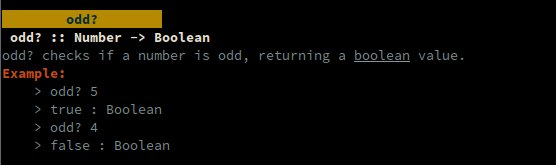
\includegraphics[width=\textwidth]{images/odd.jpg}
    \caption{odd? as seen in the terminal}
\label{fig:oddterm}
\end{figure}

\begin{itemize}
    \item a \textbf{comment} begins with `(*' and ends with `*)'
    \item the \textbf{comment name} is surrounded with `=='. This is the lookup string for the repl
        search.
    \item the \textbf{repl title} is surrounded with `***'. This text will be highlighted by a yellow
        bar in the repl.
    \item text to be rendered \textbf{bold} is surrounded with `**'
    \item text to be \underline{underlined} is surrounded with `__'
    \item headers are surrounded with `\#' 
    \item plain text is left without markup.
\end{itemize}

While not enforced by the syntax itself, underlined words are those which can be found in the
glossary. The glossary is a list of words, written with this markup, which might be unfamiliar to
students.

    \chapter{Using the Repl}
    \label{appendix:repl}
    The following commands are available in the repl (Table~\ref{tabel:repl}):

\begin{table}[ht]
    \begin{tabu}{l l r}
            Command & Arguments & Purpose \\
            \hline \\
            \textit{expr} & & Evaluate an expression \\
            :t & function & Check the type of a function \\
            :? :help & function / glossary & Read the help \\
            :clear & & Clear the terminal \\
            :using & lib name & Load a module from the standard library \\
            :q :quit & & Exit microML \\
            :load & filepath & Load a script into the repl \\
            :browse & & See the functions in the environment \\
            :pst & \textit{expr} & Pretty print parse tree to terminal \\
            :pstText & \textit{expr} & Print text form of parse tree \\
            :! & string & call the shell \\
    \end{tabu}
\caption{In-repl commands}
\label{tabel:repl}
\end{table}

Interactions in the repl are \textbf{line-orientated}. Multiline input is not yet supported.

    \chapter{Code Samples}
    \label{appendix:samples}
    \subsubsection{State in the Repl}
As Haskell encapsulates state within monads, any function which seeks to manipulate state must be
within that monad. This was most important in the type inference module and in the repl, where new
function definitions had to be dynamically added to the environment and type-checked.
Figure~\ref{fig:exec}

\begin{figure}
    \begin{minted}[breaklines=true]{haskell}
        -- | execution function while repl is running
        exec :: Bool -> L.Text -> Repl ()
        exec update source = do
            st       <- get

            mod'     <- hoistError $ parseProgram "<stdin>" source
            typeEnv' <- hoistError $ inferTop (typeEnv st) mod'

            let st' = st { termEnv = foldl' evalDef (termEnv st) mod'
                         , typeEnv = typeEnv' `mappend` typeEnv st 
                         }

            when update (put st')

            case Prelude.lookup "it" mod' of
              Nothing -> return ()
              Just ex -> do
                let (val, _) = runEval (termEnv st') "it" ex
                showOutput val st'
    \end{minted}
    \caption{The exec function in Repl.Repl}
\label{fig:exec}
\end{figure}

\subsubsection{Type checking of built-in functions}
Primitive operators and functions, such as head and tail are not available to the inference engine.
Therefore it was necessary to `hard code' the type signatures into the environment, thereby allowing
students to check the type signature of various important functions, but also meaning that these
functions can now be type checked\footnote{Haskell overcomes this problem partially by having almost
everything as a library function, including such things as + and -, which in microML are
primitives.}. Figure~\ref{fig:typesigs}

\begin{figure}
    \begin{minted}[breaklines=true]{haskell}
          ("show"   , Forall  [polyA] (TVar polyA `TArrow` typeString))
        , ("read"   , Forall  [] (typeString `TArrow` typeNum))
        , ("ord"    , Forall  [] (typeChar `TArrow` typeNum))
        , ("chr"    , Forall  [] (typeNum `TArrow` typeChar))
    \end{minted}
    \caption{Hard-coded type signatures, in Data.Map form}
\label{fig:typesigs}
\end{figure}

\subsubsection{A Parsec Parser Combinator}
An example of a typical parsing function. Complex regular expressions have been replaced with small
regular expressions and other parser combinators. Figure~\ref{fig:parsec}

\begin{figure}
    \begin{minted}{haskell}
        lambda :: Parser Expr
        lambda = do
            reservedOp "\\"
            args <- many varName
            reservedOp "->"
            body <- expr
            return $ foldr Lam body args
    \end{minted}
    \caption{The parser for microML anonymous functions}
\label{fig:parsec}
\end{figure}

Truncating floating-point representation in the repl is done using string manipulation. The choice
of three consecutive 0s is largely arbitrary. See Figure~\ref{fig:trunc} and
Section~\ref{floatingPoint}.
\begin{figure}
    \begin{minted}[breaklines=true]{haskell}
        truncate' :: Double -> Double
        truncate' = read . dropZeros . show
            where dropZeros x = head (split x) ++ "." ++ getValid (head (tail (split x)))
                  split       = splitOn "."
                  getValid s 
                      | "e" `isInfixOf` s  = s
                      | hasform s = if length s == 1 then s else  show $ read [head s] + 1
                      | take 3 s   == "000" = "0"
                      | otherwise  = head s : getValid (tail s) 

        hasform :: String -> Bool
        hasform (_:ys) = all (== '9') ys 
    \end{minted}
    \caption{The truncation function for doubles in the repl}
\label{fig:trunc}
\end{figure}

\subsubsection{Unit Testing}
Unit testing was conducted with the HSpec package\footnote{\url{https://hspec.github.io/}}.
Figure~\ref{fig:unit}

\begin{figure}
    \begin{minted}[breaklines=true]{haskell}
        listprims :: IO ()
        listprims = hspec $ 
            describe "listprims" $ do
                describe "car" $ do
                    it "gets the head of a list" $ 
                        car (BinOp OpCons (Lit (LInt 3)) Nil) `shouldBe` (Lit (LInt 3) :: Expr)
                    it "gets the head of a string" $
                        car (Lit (LString "hello")) `shouldBe` (Lit (LChar 'h') :: Expr)
                    it "should fail on non-list ints" $ 
                        evaluate (car (Lit (LInt 1)))        `shouldThrow` anyException
                    it "should fail on non-list doubles" $ 
                        evaluate (car (Lit (LDouble 1)))     `shouldThrow` anyException
                    it "should fail on non-list chars" $ 
                        evaluate (car (Lit (LChar 'a')))     `shouldThrow` anyException
                    it "should fail on non-list bools" $ 
                        evaluate (car (Lit (LBoolean True))) `shouldThrow` anyException
    \end{minted}
    \caption{Unit testing}
\label{fig:unit}
\end{figure}


\section{Utilities}
MicroML also ships with a number of utility scripts.

The installation script is written in bash\footnote{The script makes use of bash arrays so it is not
100\% posix compatible. As \textit{dash} has now become the standard shell on Ubuntu future
iterations might need to take this into account.}. Figure~\ref{fig:installation}
\begin{figure}
    \begin{minted}[breaklines=true]{bash}
        function join_by { local IFS="$1"; shift; echo "$*"; }

        ## check for this software. Only stack is essential
        stack=$(which stack 2>/dev/null) 
        fig=$(which figlet 2>/dev/null)
        cow=$(which cowsay 2>/dev/null)
        lol=$(which lolcat 2>/dev/null)


        if [ ! -x "$fig" ]; then
            progs=("${progs[@]}" "figlet ")
        fi

        if [ ! -x "$cow" ]; then
            progs=("${progs[@]}" " cowsay ")
        fi

        if [ ! -x "$lol" ]; then
            progs=("${progs[@]}" " lolcat")
        fi

        if [ -x "$stack" ]; then
            printf "\e[1mstack found\e[0m\n"
            printf "\e[1mrunning tests and building\e[0m\n"
            stack test 
            rc=$?
            if [ "$rc" != 0 ]; then
                printf "\n\e[31mCould not pass all tests. The build has failed\e[0m\n"
                exit "$rc" 
            fi
            printf "\e[1minstalling in %s/.local/bin/\n" "$HOME"
            stack install
            rc=$?
            if [ "$rc" != 0 ]; then
                printf "\nCould not install the executable into %s/.local/bin. Please copy it manually into your path\n" "$HOME"
                exit "$rc"
            fi
            printf "\n\e[1mcopying standard libraries to home directory\e[0m\n"

            ## delete old standard libs if they are found
            if [ -x "$HOME"/.microML ]; then
                printf "\n\e[1mremoving old standard library\e[0m\n"
                rm -rf "$HOME"/.microML
            fi
            printf "\n\e[1minstalling standard library\e[0m\n"

            cp -vr src/Libs "$HOME"
            mv "$HOME/Libs" "$HOME/.microML"
            printf "\n\e[1mcopying default .microMLrc to home directory\e[0m\n"

            cp -v utils/microMLrc "$HOME"/.microMLrc
            printf "\n\e[1mfinished!\e[0m\n"

            if [ -n "$progs" ]; then
                len=${#progs[@]}
                if [ "$len" -eq 1 ]; then
                    str="${progs[*]}"
                elif [ "$len" -eq 2 ]; then
                    str=$(join_by $"&" "${progs[@]}")
                else 
                    str=$("figlet, cowsay and lolcat")
                fi
                #str=$(join_by , "${progs[@]}")
                printf "\e[1mYou can have a more interesting repl if you also install %s\e[0m\n" "$str"
            fi
        else 
            printf "\e[31mCould not find stack in your system path. Please install it using your package
            manager or go to \e[0;1mhttps://docs.haskellstack.org/en/stable/README/\e[0m\n"
        fi
    \end{minted}
    \caption{Bash installation script}
\label{fig:installation}
\end{figure}

MicroML also has a simple (neo)vim plugin which ships with the repo. The folding function is of some
interest, as it autofolds comments, setting the function name as its `title'. See
Figures~\ref{fig:fold} and~\ref{fig:foldVim}

\begin{figure}
    \begin{minted}[breaklines=true]{vim}
        function! GetMMLFold(lnum) 
            let l:line = getline( a:lnum )

            " Beginning of comment
            if l:line =~? '\v^\s*--' || l:line =~? '\v^\s*(\*'
                return '2'
            endif

            if l:line =~? '\v^\s*$'
                let l:nextline = getline(a:lnum + 1)
                if l:nextline =~# '^--' || l:nextline =~? '^(\*'
                    return '0'
                else
                    return '-1'
                endif
            endif
            return '1'
        endfunction 
    \end{minted}
    \caption{Part of the folding function for vim}
\label{fig:fold}
\end{figure}

    \chapter{Diary}
    \label{appendix:diary}
    \section{Formalities} 

\textbf{Thursday 26 May}  --- Dean asks about group.  \\
\textbf{Friday 27 May}  --- inducted into micro:bit team \\
               --- Dean confirms functional project as carte blanche \\
--- start research into an ml style language \\
\textbf{Saturday 28 May}  --- decide to target micropython with a Haskell compiler \\
\textbf{Sunday 29 May}  --- comparison of functional languages \\
\textbf{Tuesday 31 May}  --- meeting with Rae at 2:30 \\
\textbf{}  --- discussed making a dsl for micro:bit. Need to justify educational value. \\
\textbf{}  --- Focus on robotics. Wants a doc detailing requirements and constraints of design. \\
\textbf{Wednesday 1 June}  --- started drafting initial report for Rae and Peli. Hope to send tomorrow \\
\textbf{Thursday 2 June}  --- sent initial proposal to Rae and Peli \\

\section{Project Start} 

\textbf{Wednesday 8 June}  --- finally hear from Rae, who is happy with the proposal. Still no word from Peli. \\
\textbf{}  --- meeting scheduled for tomorrow morning. \\
\textbf{}  --- Started tutorial for CoreLang (SPJ) which looks a promising base for microML \\
\textbf{Thursday 9 June}  --- morning meeting with Rae, details of which (prepare examples of
backends) are superseded by emails from Peli and Tom Ball, recommending using the C++ API as target language. \\
\textbf{Friday 10 June}  --- started work in microML parser. Research Text.Indentation and Trifecta \\
\textbf{Sunday 12 June}  --- basic work on simple parser and repl done. Only parses one line of input. \\
\textbf{Monday 13 June}  --- started rewriting using megaparsec. Good progress made. Reused repl code \\
\textbf{Tuesday 14 June}  --- implemented lambda parsing and most of type signature parsing. Indentation still to do \\
\textbf{Wednesday 15 June}  --- tuples added to parser and type signatures fixed. Type aliasing added. File reading still not working \\
\textbf{Thursday 16 June}  --- more work on parser \\
\textbf{Friday 17 June}  --- started work on evaluation for repl. Arithmetic done and simple boolean operators \\
\textbf{Monday 20 June}  --- little progress. Still can't store values in the repl \\
\textbf{Tuesday 21 June}  --- started refactoring code, removing all problematic elements \\
\textbf{Wednesday 22 June}  --- repl finally working, moving on to type inference \\
\textbf{Thursday 23 June}  --- starting writing tests, using Hspec, for parser/lexer \\
\textbf{Friday 24 June}  --- recursion now working, but syntax needs to be improved \\
\textbf{Monday 27 June}  --- working on pattern matching and simple type inference \\
\textbf{Tuesday 28 June}  --- as above \\
\textbf{Wednesday 29 June}  --- simple type inference almost working but needs to be extended. Pattern matching parser working, \\
                    but no supporting algorithm of language support yet. \\
\textbf{Thursday 30 June}  --- fixed type inference for numbers (a slight hack here, only allowing a Num type) \\
\textbf{Friday 1 July}  --- working on lists. Need to rewrite the interpreter. Then finish on this part. Removed pattern matching.  \\
                    Simplified pretty printer. \\
\textbf{Monday 4 July}  --- recursion on lists is finally working. Once type inference on lists work, we can move on to compilation \\
\textbf{Tuesday 5 July}  --- cons operator is working. Now only list type inference is major outstanding feature of repl. \\
\textbf{Wednesday 6 July}  --- type inference now working on lists. Started writing Github wiki. \\
\textbf{Thursday 7 July}  --- meeting with Rae. Agreed to start writing up progress. Start debugging. \\
\textbf{Monday 11 July}  --- exception handling added to inference module, not yet complete \\
\textbf{Wednesday 13 July}  --- refactored primitive ops so that sqrt and others are now properly typechecked \\
\textbf{Thursday 14 July}  --- very little done. Meeting with Rae. ord, chr, toUpper and toLower. Start of string library \\
\textbf{Friday 15 July}  --- added command line arguments to main program. Successfully compiled hello world! \\
\textbf{Sunday 17 July}  --- fixed bug in string literal printing \\
\textbf{Tuesday 19 July}  --- started work on new version of compiler. Simple functions work \\
\textbf{Wednesday 20 July}  --- finally starting to understand Monad transformers after doing
tutorial. Added ExceptT to compiler module :) \\
\textbf{Thursday 21 July}  --- started adding type inference to compiler. Lots of small bugs fixed. \\
\textbf{Friday 22 July}  --- more error handling, for mod, head and tail, also ord and chr (though they can't be typechecked) \\
\textbf{Monday 25 July}  --- finally fixed list type inference, including nested lists \\
\textbf{Tuesday 26 July}  --- fixed pretty printing of lists. Standard library typechecks but is too general. \\
\textbf{Monday 1 August}  --- type inference also completely fixed. Only lists left to go (or so it seems) \\
\textbf{Tuesday 2 August}  --- lists still not working as expected. A slow day \\
\textbf{Wednesday 3 August}  --- fresh start on compiler. Good progress made with error messages. \\
\textbf{Thursday 4 August}  --- started working on elixir style docs. Wrote small markdown parser \\
\textbf{Friday 5 August}  --- numerous small bug fixes, but docs not quite working yet. Must move on to compiler!! \\
\textbf{Monday 8 August}  --- docs fixed. Compiler now refuses to compile if main is missing, or if there are \\
                    duplicate definitions, or if a function is unreachable. All with appropriate error messages. Shell \\
                    escape in repl now has proper error handling. :clear added as independent function. Wrote docs for standard.mml \\
                    Removed some unreachable code from Infer.hs and improved error handling. A good day. \\
\textbf{Tuesday 9 August}  --- little progress made. Abandoning c-dsl \\
\textbf{Wednesday 10 Aug}  --- new version of compiler started, much simpler but appears to be working. Also \\
                   added typesigs for built-in functions  --- this might be a good way to infer lambdas \\
\textbf{Thursday 11 Aug}  --- improved callgraph. Changed to using stack as a build tool. Had to remove llvm \\
                     as a result \\
\textbf{Friday 12 Aug}  --- restarted compiler again, this time using ExceptT and monad stack (as per transformers tutorial) \\
\textbf{Monday 15 Aug}  --- using RWST for compiler. Added dotfile production of callgraph. Compiler (though primitive) working as proof of concept. \\
\textbf{Tuesday 16 Aug}  --- added pst command, with a nice pretty printed parse tree in the repl,
complete with error handling. \\
\textbf{Wednesday 17 Aug}  --- added clang  ---format for file. Added typeEnv into Compiler monad, but not yet working as expected \\
\textbf{Thursday 18 Aug}  --- wrote folding method for microML in vim. Started write up of report \\
\textbf{Friday 19 Aug}  --- worked on report. Used tikz for the first time in latex. \\
\textbf{Monday 22 Aug}  --- worked on report \\
\textbf{Tuesday 23 Aug}  --- worked on report. Wrote simple bash script to run compiler tests. Wrote unit \\
                   tests for ListPrimitives. Bash script to compile latex with bibliography \\
\textbf{Wednesday 24 Aug}  --- writing \\

\end{appendices}

%% check this list to make sure things have been cited
\nocite{adams2012layout}
\nocite{9780511608865}
\nocite{Wadler:1995:MFP:647698.734146}
\nocite{958}
\nocite{Steele:1994:BIC:174675.178068}
\nocite{opac-b1081362}

\bibliography{bibliography}{}
\bibliographystyle{plain}
\end{document}
